\documentclass[tikz,border=12pt]{standalone}

\usepackage[utf8]{inputenc}
\usepackage{amsmath}
\usepackage{tikz}
\usetikzlibrary{arrows.meta,positioning,fit,backgrounds,calc}

% =========================================================
% RT-HBTNet architecture figure - revised architecture only
% =========================================================

% -------------------------
% Colors
% -------------------------
\definecolor{cBlueF}{RGB}{214,232,252}
\definecolor{cBlueB}{RGB}{30,95,170}
\definecolor{cAmberF}{RGB}{254,228,160}
\definecolor{cAmberB}{RGB}{155,95,10}
\definecolor{cGreenF}{RGB}{195,238,180}
\definecolor{cGreenB}{RGB}{45,135,45}
\definecolor{cTealF}{RGB}{180,235,220}
\definecolor{cTealB}{RGB}{15,105,85}
\definecolor{cPurpleF}{RGB}{220,212,252}
\definecolor{cPurpleB}{RGB}{75,55,175}
\definecolor{cCoralF}{RGB}{252,210,195}
\definecolor{cCoralB}{RGB}{175,65,35}
\definecolor{cGrayF}{RGB}{232,230,224}
\definecolor{cGrayB}{RGB}{110,108,100}
\definecolor{texBranch}{RGB}{232,243,255}
\definecolor{blurBranch}{RGB}{255,247,228}
\definecolor{ctxBg}{RGB}{255,236,226}
\definecolor{fusionBg}{RGB}{238,234,255}
\definecolor{stabBg}{RGB}{230,248,240}
\definecolor{encBg}{RGB}{232,248,238}

% -------------------------
% Styles
% -------------------------
\tikzset{
  nd/.style={
    rectangle,
    rounded corners=4pt,
    minimum width=#1,
    minimum height=1.05cm,
    text width=#1,
    align=center,
    font=\fontsize{8}{9.5}\selectfont\sffamily,
    line width=0.65pt,
    inner sep=4pt
  },
  nd/.default=2.35cm,
  bluend/.style={nd=#1, fill=cBlueF, draw=cBlueB},
  bluend/.default=2.35cm,
  ambernd/.style={nd=#1, fill=cAmberF, draw=cAmberB},
  ambernd/.default=2.35cm,
  greennd/.style={nd=#1, fill=cGreenF, draw=cGreenB},
  greennd/.default=1.85cm,
  tealnd/.style={nd=#1, fill=cTealF, draw=cTealB},
  tealnd/.default=2.15cm,
  purplend/.style={nd=#1, fill=cPurpleF, draw=cPurpleB},
  purplend/.default=3.05cm,
  coralnd/.style={nd=#1, fill=cCoralF, draw=cCoralB},
  coralnd/.default=2.4cm,
  graynd/.style={nd=#1, fill=cGrayF, draw=cGrayB},
  graynd/.default=2.0cm,
  arr/.style={-{Stealth[length=5pt,width=4pt]}, line width=0.75pt},
  dasharr/.style={arr, dashed, dash pattern=on 3pt off 2.2pt},
  cont/.style={
    rectangle,
    rounded corners=7pt,
    dashed,
    line width=0.8pt,
    inner sep=12pt
  },
  lab/.style={font=\fontsize{8.2}{9.5}\selectfont\sffamily\bfseries}
}

\begin{document}
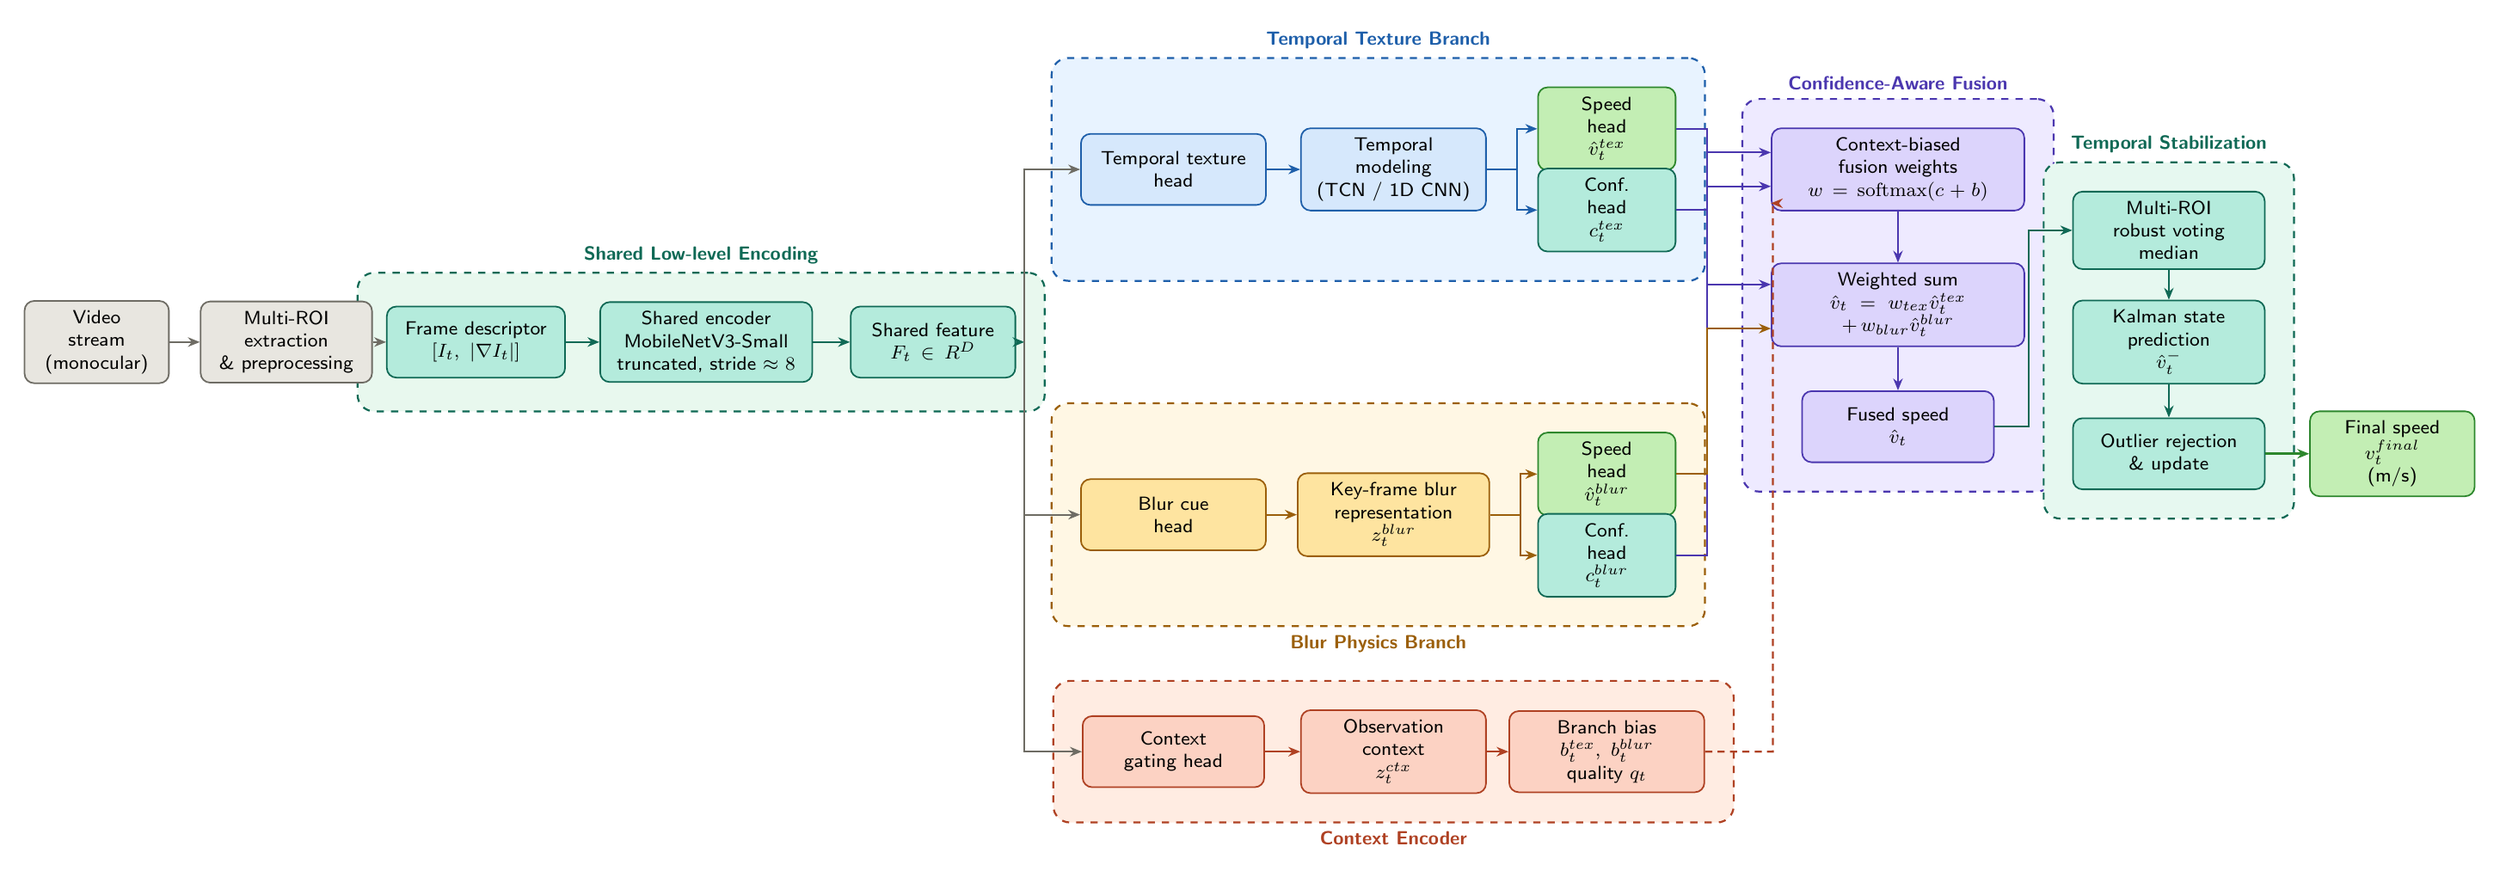
\begin{tikzpicture}[x=1cm,y=1cm]

% =========================================================
% Input, ROI, shared descriptor and encoder
% =========================================================
\node[graynd=1.85cm] (video) at (-0.35,0)
  {Video\\stream\\(monocular)};

\node[graynd=2.25cm] (roi) at (2.45,0)
  {Multi-ROI\\extraction\\\& preprocessing};

\node[tealnd=2.35cm] (desc) at (5.25,0)
  {Frame descriptor\\$[I_t,\ |\nabla I_t|]$};

\node[tealnd=2.85cm] (shared_enc) at (8.65,0)
  {Shared encoder\\MobileNetV3-Small\\truncated, stride $\approx 8$};

% FIX 1: \mathbb{R} must not be split across lines
\node[tealnd=2.15cm] (shared_feat) at (12.0,0)
  {Shared feature\\$F_t \in \mathbb{R}^{D}$};

\draw[arr, color=cGrayB] (video.east) -- (roi.west);
\draw[arr, color=cGrayB] (roi.east) -- (desc.west);
\draw[arr, color=cTealB] (desc.east) -- (shared_enc.west);
\draw[arr, color=cTealB] (shared_enc.east) -- (shared_feat.west);

\begin{scope}[on background layer]
  \node[cont, fill=encBg, draw=cTealB,
        fit=(desc)(shared_enc)(shared_feat),
        label={[lab, color=cTealB]above:Shared Low-level Encoding}] (encBox) {};
\end{scope}

% Split point after shared encoder.
\coordinate (split) at (13.35,0);
\draw[arr, color=cTealB] (shared_feat.east) -- (split);

% =========================================================
% Temporal Texture Branch
% =========================================================
\node[bluend=2.45cm] (tex_head) at (15.55,2.55)
  {Temporal texture\\head};

\node[bluend=2.45cm] (tcn) at (18.8,2.55)
  {Temporal\\modeling\\(TCN / 1D CNN)};

\node[greennd=1.75cm] (spd_tex) at (21.95,3.15)
  {Speed\\head\\$\hat{v}^{tex}_t$};

\node[tealnd=1.75cm] (conf_tex) at (21.95,1.95)
  {Conf.\\head\\$c^{tex}_t$};

\draw[arr, color=cGrayB] (split) |- (tex_head.west);
\draw[arr, color=cBlueB] (tex_head.east) -- (tcn.west);
\draw[arr, color=cBlueB] (tcn.east) -- ++(0.45,0) |- (spd_tex.west);
\draw[arr, color=cBlueB] (tcn.east) -- ++(0.45,0) |- (conf_tex.west);

% =========================================================
% Blur Physics Branch
% =========================================================
\node[ambernd=2.45cm] (blur_head) at (15.55,-2.55)
  {Blur cue\\head};

\node[ambernd=2.55cm] (blur_latent) at (18.8,-2.55)
  {Key-frame blur\\representation\\$z^{blur}_t$};

\node[greennd=1.75cm] (spd_blur) at (21.95,-1.95)
  {Speed\\head\\$\hat{v}^{blur}_t$};

\node[tealnd=1.75cm] (conf_blur) at (21.95,-3.15)
  {Conf.\\head\\$c^{blur}_t$};

\draw[arr, color=cGrayB] (split) |- (blur_head.west);
\draw[arr, color=cAmberB] (blur_head.east) -- (blur_latent.west);
\draw[arr, color=cAmberB] (blur_latent.east) -- ++(0.45,0) |- (spd_blur.west);
\draw[arr, color=cAmberB] (blur_latent.east) -- ++(0.45,0) |- (conf_blur.west);

% =========================================================
% Containers behind top branches
% =========================================================
\begin{scope}[on background layer]
  \node[cont, fill=texBranch, draw=cBlueB,
        fit=(tex_head)(tcn)(spd_tex)(conf_tex),
        label={[lab, color=cBlueB]above:Temporal Texture Branch}] (texBox) {};

  \node[cont, fill=blurBranch, draw=cAmberB,
        fit=(blur_head)(blur_latent)(spd_blur)(conf_blur),
        label={[lab, color=cAmberB]below:Blur Physics Branch}] (blurBox) {};
\end{scope}

% =========================================================
% Context Encoder
% =========================================================
\node[coralnd=2.4cm] (ctx_enc) at (15.55,-6.05)
  {Context\\gating head};

\node[coralnd=2.45cm] (ctx_feat) at (18.8,-6.05)
  {Observation\\context\\$z^{ctx}_t$};

\node[coralnd=2.6cm] (ctx_scores) at (21.95,-6.05)
  {Branch bias\\$b^{tex}_t,\ b^{blur}_t$\\quality $q_t$};

\draw[arr, color=cGrayB] (split) |- (ctx_enc.west);
\draw[arr, color=cCoralB] (ctx_enc.east) -- (ctx_feat.west);
\draw[arr, color=cCoralB] (ctx_feat.east) -- (ctx_scores.west);

\begin{scope}[on background layer]
  \node[cont, fill=ctxBg, draw=cCoralB,
        fit=(ctx_enc)(ctx_feat)(ctx_scores),
        label={[lab, color=cCoralB]below:Context Encoder}] (ctxBox) {};
\end{scope}

% =========================================================
% Confidence-Aware Fusion
% =========================================================
\node[purplend=3.45cm] (fusion_mlp) at (26.25,2.55)
  {Context-biased\\fusion weights\\$w=\mathrm{softmax}(c+b)$};

\node[purplend=3.45cm] (wsum) at (26.25,0.55)
  {Weighted sum\\$\hat{v}_t=w_{tex}\hat{v}^{tex}_t$\\$+\,w_{blur}\hat{v}^{blur}_t$};

\node[purplend=2.55cm] (fused) at (26.25,-1.25)
  {Fused speed\\$\hat{v}_t$};

\begin{scope}[on background layer]
  \node[cont, fill=fusionBg, draw=cPurpleB,
        fit=(fusion_mlp)(wsum)(fused),
        label={[lab, color=cPurpleB]above:Confidence-Aware Fusion}] (fusionBox) {};
\end{scope}

% Separate lane coordinates before fusion.
\coordinate (confTexLane)  at (24.00,2.80);
\coordinate (confBlurLane) at (24.25,2.30);
\coordinate (ctxLane)      at (24.50,2.05);
\coordinate (spdTexLane)   at (24.00,0.85);
\coordinate (spdBlurLane)  at (24.25,0.20);

% Confidence heads and context bias to fusion weights.
\draw[arr, color=cPurpleB] (conf_tex.east) -- ++(0.45,0) |- (confTexLane) -- (fusion_mlp.west |- confTexLane);
\draw[arr, color=cPurpleB] (conf_blur.east) -- ++(0.45,0) |- (confBlurLane) -- (fusion_mlp.west |- confBlurLane);

\draw[dasharr, color=cCoralB]
  (ctx_scores.east) -- ++(1.00,0)
  -- ++(0,8.10)
  -- (fusion_mlp.west |- ctxLane);

% Speed heads to weighted sum.
\draw[arr, color=cPurpleB] (spd_tex.east) -- ++(0.45,0) |- (spdTexLane) -- (wsum.west |- spdTexLane);
\draw[arr, color=cAmberB]  (spd_blur.east) -- ++(0.45,0) |- (spdBlurLane) -- (wsum.west |- spdBlurLane);

% Internal fusion flow.
\draw[arr, color=cPurpleB] (fusion_mlp.south) -- (wsum.north);
\draw[arr, color=cPurpleB] (wsum.south) -- (fused.north);

% =========================================================
% Temporal Stabilization
% =========================================================
\node[tealnd=2.55cm] (roi_vote) at (30.25,1.65)
  {Multi-ROI\\robust voting\\median};

% FIX 2: (state_pred) node was missing its content and semicolon entirely
\node[tealnd=2.55cm] (state_pred) at (30.25,0.0)
  {Kalman state\\prediction\\$\hat{v}^{-}_t$};

\node[tealnd=2.55cm] (meas_upd) at (30.25,-1.65)
  {Outlier rejection\\\& update};

\begin{scope}[on background layer]
  \node[cont, fill=stabBg, draw=cTealB,
        fit=(roi_vote)(state_pred)(meas_upd),
        label={[lab, color=cTealB]above:Temporal Stabilization}] (stabBox) {};
\end{scope}

\draw[arr, color=cTealB] (fused.east) -- ++(0.50,0) |- (roi_vote.west);
\draw[arr, color=cTealB] (roi_vote.south) -- (state_pred.north);
\draw[arr, color=cTealB] (state_pred.south) -- (meas_upd.north);

% =========================================================
% Output
% =========================================================
\node[greennd=2.15cm] (output) at (33.55,-1.65)
  {Final speed\\$v^{final}_t$\\(m/s)};

\draw[arr, color=cGreenB, line width=0.95pt] (meas_upd.east) -- (output.west);

\end{tikzpicture}
\end{document}